The firmware was split into a number of separate modules, as shown in Figure
\ref{fig:fw_block_diag}. All of the drivers for microcontroller peripherals,
such as serial interfaces and the ADC are provided by the nRF52 SDK's hardware
abstraction layer. Some higher level components from the
nRF52 SDK such as the USB CDC-ACM stack, a FAT32 filesystem driver and Nordic's
soft device 140 which is a Bluetooth LE peripheral stack are also used.

These third party components will be used by the software coded in-house,
which includes the drivers for all the sensors (IMU, optical
heart rate sensor, air quality sensor and UV light sensor) as well as the signal
processing code required to derive a heart rate from the raw data we receive
from our optical heart rate sensor. While we plan to use a third party file
system implementation, we will still need to write the code that allows blocks
to be written to and read from an SD card over an SPI interface.

At the application layer we have three modules. Our data logging service will be
responsible for most of the operation of our device and will continually collect
and log sensor data. The Bluetooth data transfer service will facilitate
accessing the logged data over a Bluetooth interface. Our debugging interface is
intended to expose our firmware functionality over a USB serial interface so
that integration tests can be run on the microcontroller. A block diagram of the 
firmware is shown below in Figure…

\begin{figure}[!htb]
\centering
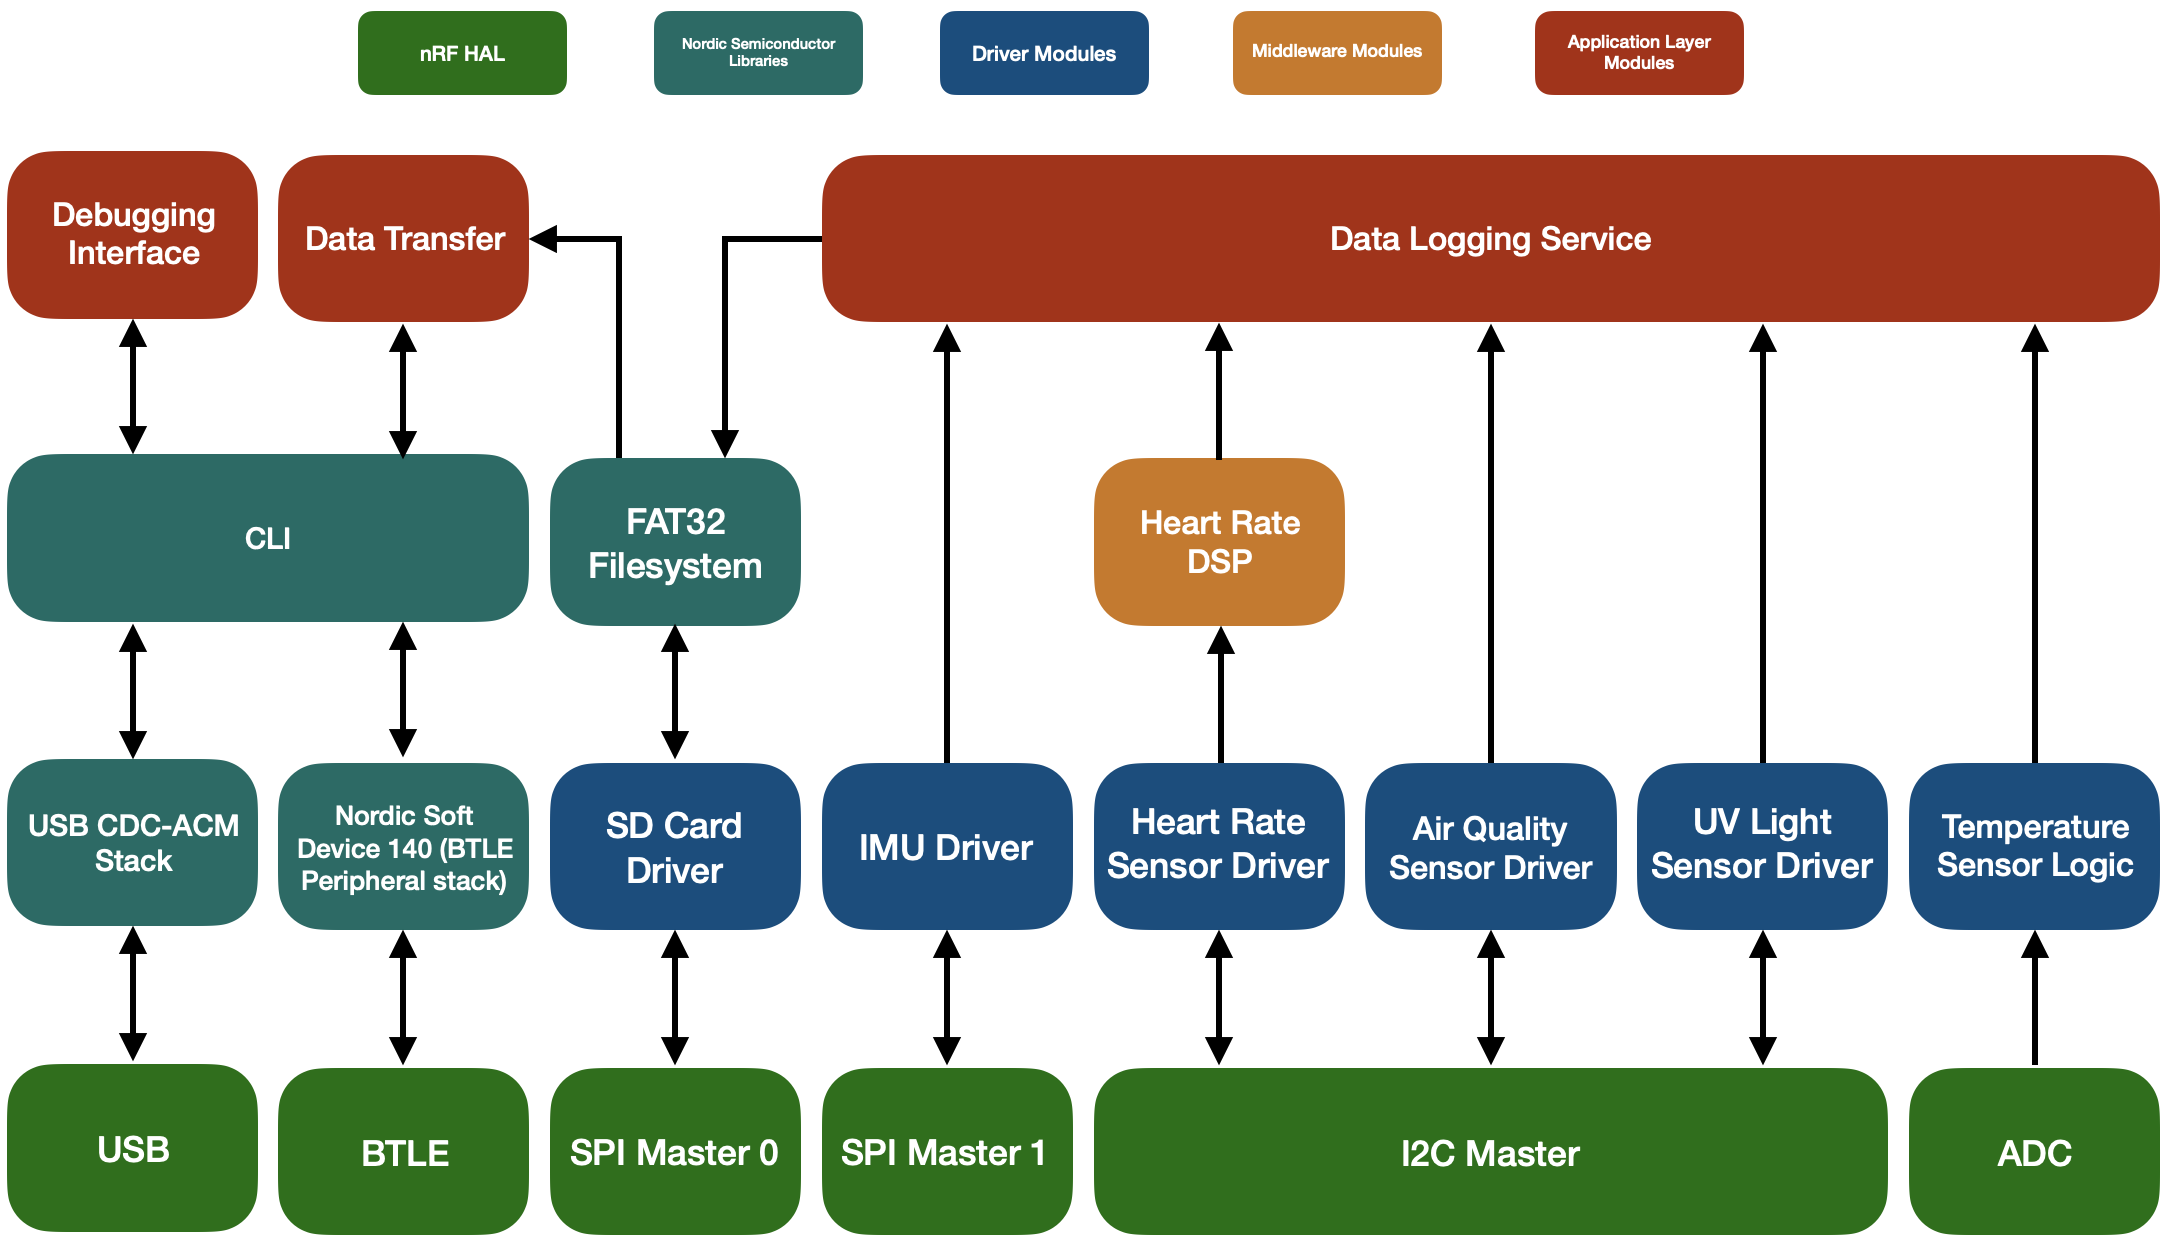
\includegraphics[width=\textwidth]{images/fw_block_diag.png}
\caption{Firmware block diagram.}
\label{fig:fw_block_diag}
\end{figure}

While considering operating systems to use, we came to the conclusion 
that most of the benefits of using a RTOS 
%again, define RTOS
are unnecessary for our application.
Because most of the sensors have internal buffers, we can periodically poll
for data without needing formal scheduling pattern. Other features of 
operating systems such as memory management or preemption would not be
necessary, as the services handling reading the sensor data and logging
to the SD card using co-operative multi-tasking will be sufficient and require
less effort and are less risky compared to using an RTOS.

The software was written on the bare metal and follows a structure where there
is a central loop which calls services for all components.  Each sensor as well
as the data logging component are implemented as a separate component
to be updated periodically. The drivers read and process the data from the
sensors and write it to a buffer to be written to the SD card. The logging service
maintains a few of these buffers and ensures they are written to the SD card
at reasonable intervals.

\subsection{Drivers}

\subsubsection{USB}

\subsubsection{Bluetooth}

The design goal for the Bluetooth driver was to have it mimic a serial
port in the same fashion that USB CDC does. Our intention was to 
simplify the design of the companion software as well as the command line 
interface present on the microcontroller. This goal was fully achieved 
on the microcontroller side of the communication link. The software interface for 
Bluetooth was made identical to USB so that they can be used interchangeably 
without additional complications. On the PC side where the companion software
runs, the solution was not as elegant. We had hoped to find a way to make the
Bluetooth connection appear as a serial port so it could be used interchangeably
with the USB CDC connection, but a method to implement this could not be determined. It 
could likely be accomplished by writing custom drivers, but this was outside the scope of the
project. Instead, a cross-platform Python library was used to establish the
Bluetooth connection to the device and communicate with it as would a Bluetooth device.

The device uses Bluetooth Low Energy, which works by advertising
available services to other nearby devices. Each service may offer a number
of characteristics that can be read only, write only, read-write, and have 
several other options such as notifying a connected device when a characteristic
value changes. The Bluetooth Low Energy specification includes descriptions of several
standard services and their characteristics, but none of these could be used to
to achieve the serial port-like behaviour needed for this project. A custom
serial port service included with the Nordic SDK was used instead. This service
has two characteristics, one named TX and one named RX. The RX characteristic is
write only and is used to send data to the device. The TX characteristic is
written to only by the device and has notifications enabled. If a connected device
wants to receive data then it must subscribe to the notifications of the TX 
characteristic. This solution worked quite well, although it has a low 
throughput in comparison to USB. The fact that each notification packet can only 
hold approximately 20 bytes and must be acknowledged before the next one is 
sent likely contributes significantly to the low throughput. However, it was not expected
that Bluetooth Low Energy would be very fast since it is optimized for 
power consumption instead of speed. This trade-off is well suited to this project 
because it is battery powered.

\subsubsection{Heart Rate}

Our heart rate driver is based on an open source implementation written in
C++ \cite{max86150-ardino}. Since the SDK 
%please again define SDK
we are using falls under the nRF5
Nordic License, only software that is compatible with this license can be
integrated into the project. The open source C++ heart rate driver is under the
expat license so we are free to use it as long as the copyright notice is
maintained. Unfortunately, not all useful open source software was licensed in
a way compatible with the SDK license. In particular, it would have been ideal
to reuse an algorithm to convert raw PPG data to beats per minute, however the
available algorithm was licensed with the Lesser GNU Public
License \cite{wasp-os} which is incompatible with the SDK license.
